% Este modelo de apresentação de TCC é baseado no trabalho de Lima (2023). Mantenha este comentário no topo do arquivo.
\documentclass[11pt]{beamer}
\usetheme{Madrid}

\definecolor{islamicgreen}{rgb}{0.0, 0.46, 0.1}
\setbeamercolor{palette primary}{bg=islamicgreen,fg=white}
\setbeamercolor{palette secondary}{bg=islamicgreen,fg=white}
\setbeamercolor{palette tertiary}{bg=islamicgreen,fg=white}
\setbeamercolor{palette quaternary}{bg=islamicgreen,fg=white}
\setbeamercolor{structure}{fg=islamicgreen}
\setbeamercolor{section in toc}{fg=black} 

\usepackage[utf8]{inputenc}
% Comentado para evitar erro caso o pacote de idioma não esteja instalado no TeX Live do sistema
% \usepackage[brazilian]{babel}
\usepackage{amsmath}
\usepackage{amsfonts}
\usepackage{amssymb}
\usepackage{booktabs,tabularx}
\usepackage{array}
\newcolumntype{L}[1]{>{\raggedright\arraybackslash}p{#1}}
\usepackage{csquotes}
\usepackage{graphicx}
\usepackage{longtable}
\usepackage{mathptmx}
\usepackage{multirow}
\usepackage{tikz}
\usetikzlibrary{arrows.meta}
\usepackage[
    backend=biber,
    style=numeric-comp,
]{biblatex}
\makeatletter
\hypersetup{
	pdftitle={\@title}, 
	pdfauthor={André Vitor Bastos de Macêdo},
	pdfsubject={Trabalho de Conclusão de Curso submetido ao Curso de Bacharelado em Ciência da Computação do Instituto Federal Catarinense — \textit{Campus} Blumenau para a obtenção do título de Bacharel em Ciência da Computação.},
	pdfcreator={PDFLaTeX with beamer},
	pdfkeywords={tcc, ia, pathfinding, bcc, ifc, latex, beamer}, 
}
\makeatother

\renewcommand*{\bibfont}{\normalfont\tiny}
\renewcommand{\indent}{\hspace*{2em}}

\makeatletter
\renewcommand\@makefntext[1]{\leftskip=2em\hskip-0.5em\@makefnmark#1}
\makeatother

\setbeamertemplate{section in toc}{
    \hspace*{1em}\inserttocsectionnumber.~\inserttocsection\par
}

\setbeamertemplate{subsection in toc}{
    \hspace*{2em}\inserttocsectionnumber.\inserttocsubsectionnumber.~\inserttocsubsection\par
}

\author{André Vitor Bastos de Macêdo \\ 
\small Orientador: Prof. Paulo César Rodacki Gomes}
\title{\textbf{Pathfinding em Malhas 3D}}
\subtitle{Análise estatística e comparativa}
\newcommand{\email}{andre.bastos@ifc.edu.br}
\setbeamercovered{transparent} 
\setbeamertemplate{navigation symbols}{} 
\setbeamertemplate{footline}[page number]
\titlegraphic{\hfill
\includegraphics[scale=0.2]{figuras/ifc-logo.png}}
\institute[]{Instituto Federal Catarinense\\Campus Blumenau} 
\date{2026} 

\addbibresource{referencias.bib}

\begin{document}

\begin{frame}
\titlepage
\end{frame}

\setcounter{tocdepth}{1}
\begin{frame}{Sumário}
\tableofcontents
\end{frame}

\section{Introdução}

\begin{frame}{Introdução e Definição do Problema}
    Busca de caminhos (ou \textit{pathfinding}) é a lógica de encontrar caminhos entre um ponto de partida e um objetivo por meio da exploração de um grafo \cite{rodacki_grafos}.
    \vspace{1.5em}
    
    De puramente abstratos para aplicação direta na computação interativa, é um componente crucial para o desenvolvimento de jogos e simulações em tempo real \cite{pathfinding_game_dev}.
\end{frame}

\begin{frame}{Introdução e Definição do Problema}
    Em espaços 2D, a passagem entre coordenadas inteiras é uniforme e fácil de se navegar.
    \vspace{1.5em}

    No espaço 3D, é preciso considerar a variação de altura, inclinação do relevo e obstáculos complexos.
    Isso traz instabilidade e inconsistências matemáticas nos cálculos de distância \cite{a_star_modification}.
    \vspace{1em}
    
    \centering
    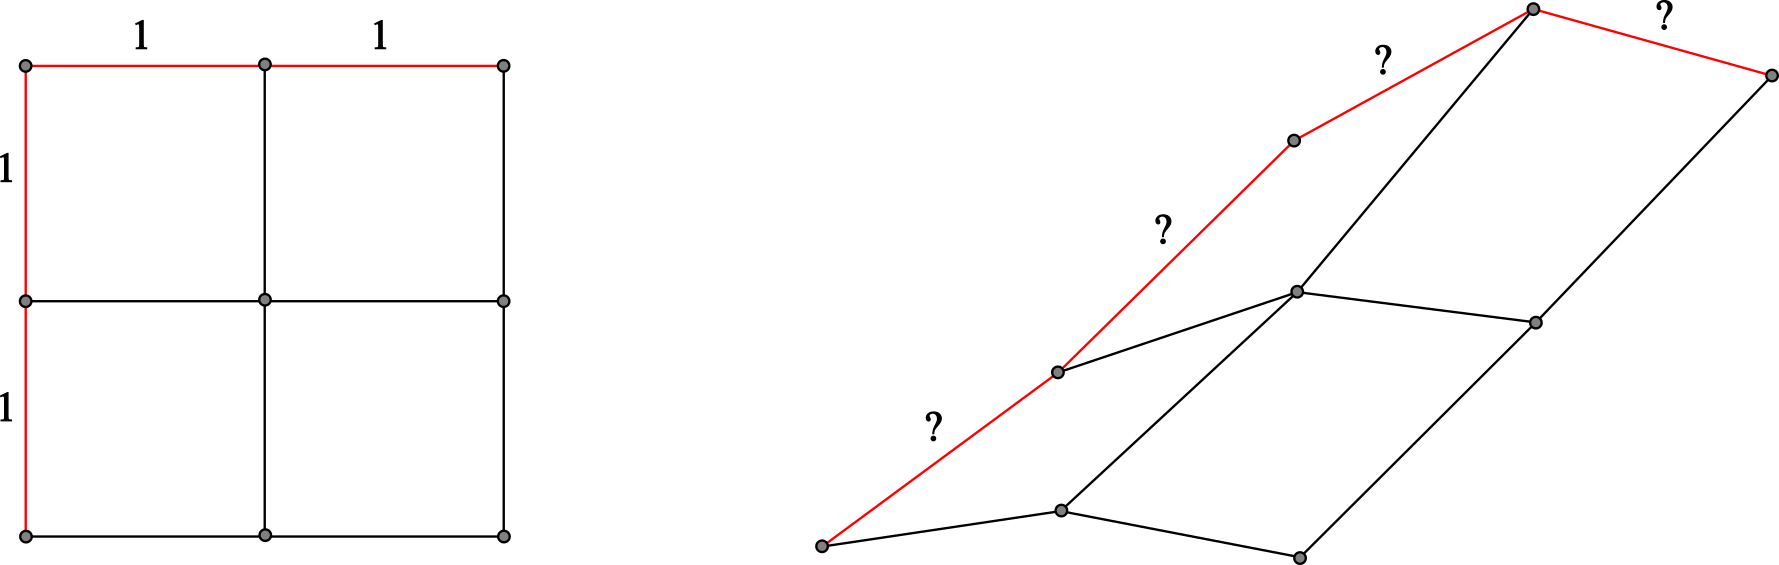
\includegraphics[width=0.7\textwidth]{figuras/2d_vs_3d.png}
\end{frame}

\section{Objetivos}

\begin{frame}{Objetivos}
    \textbf{Geral:} Analisar comparativa e estatisticamente o desempenho de algoritmos de busca altamente usados em múltiplos cenários 3D.
    \vspace{1.5em}

    \textbf{Específicos:}
    \begin{enumerate}
        \item Implementar uma biblioteca de grafos eficiente para execução de algoritmos de pathfinding.
        \item Desenvolver uma infraestrutura de renderização para visualização das malhas e caminhos encontrados.
        \item Adaptar a arquitetura para execução concorrente e testes de estresse.
        \item Desenvolver geradores procedurais de malhas para diferentes cenários de teste.
        \item Analisar estatisticamente os resultados obtidos nos testes.
    \end{enumerate}
\end{frame}

\section{Justificativa}

\begin{frame}{Justificativa}
    Existe uma grande lacuna em estudos de busca de caminhos na área de renderização 3D. Pesquisas recentes tendem a focar unicamente em ambientes 2D ou em um único modelo de interpretação de malhas, como Johansson (2024)\cite{johansson2024adapting} e Kapi (2022)\cite{Kapi2022}. Este estudo visa superar essa barreira e comparar diferentes estilos de modelagem de terreno.
    \vspace{1.5em}
    
    Adicionalmente, existe a necessidade de separar a análise comparativa dos grandes motores gráficos (Unity, Unreal e outras) e trazer uma visão única e sem ruídos em uma engine criada do zero. Isso nos permite medir a performance de CPU e memória de forma pura.
\end{frame}

\section{Trabalhos Relacionados}

\begin{frame}{Trabalhos Relacionados e Diferencial Técnico}
    \begin{table}[h]\centering
        \caption{Matriz de diferenciação técnica}\label{tab:relacionados}
        \scriptsize
        \begin{tabular}{L{2.2cm} L{2.8cm} L{2.8cm} L{2.8cm}}\toprule
        \textbf{Critérios} & \textbf{Proposta} & \textbf{Johansson (2024)\cite{johansson2024adapting}} & \textbf{Kapi (2022)\cite{Kapi2022}} \\\midrule
        Dimensão Espacial & Malhas 3D volumétricas, Octrees e Voxels & Voxels (Blocos 3D)  & Grades 2D planas \\
        \vspace{0.5em}Geometria & \vspace{0.5em}Procedural & \vspace{0.5em}Cubos fixos & \vspace{0.5em}Matrizes planas \\
        \vspace{0.5em}Algoritmos & \vspace{0.5em}Dijkstra, A*, JPS e Theta* & \vspace{0.5em}A* e Dijkstra & \vspace{0.5em}A*, JPS e Theta* \\
        \vspace{0.5em}Arquitetura & \vspace{0.5em}Paralela & \vspace{0.5em}Sequencial & \vspace{0.5em}Sequencial \\
        \vspace{0.5em}Ambiente/Carga & \vspace{0.5em}Renderização 3D concorrente & \vspace{0.5em}Execução isolada & \vspace{0.5em}Execução isolada \\
        \bottomrule
        \end{tabular}
    \end{table}
\end{frame}

\section{Referencial Teórico}

\begin{frame}{Referencial Teórico e Metodologia}
    Esta pesquisa se baseia em conceitos de grafos, algoritmos de busca, geração procedural de malhas 3D e técnicas de paralelização. A seguir, serão detalhados os principais conceitos que fundamentam o desenvolvimento do projeto.
\end{frame}

\begin{frame}{Grafos}
    \textbf{Definição matemática \cite{rodacki_grafos}:}
    \begin{equation}
        G = (V, A)
    \end{equation}
    Onde:
    \begin{itemize}
        \item $G$ é um grafo.
        \item $V$ é um conjunto de vértices (entidades individuais, ex: coordenadas).
        \item $A$ é um conjunto de arestas (ligações direcionadas ou não que carregam pesos/custos).
    \end{itemize}
    \vspace{0.8em}
    Um algoritmo de busca é o procedimento que atravessa os vértices do grafo a partir das arestas e, com seus respectivos pesos, encontra o caminho de menor custo entre dois vértices.
\end{frame}

\begin{frame}{Grafos}
    O algoritmo de Dijkstra \cite{rodacki_grafos} é o algoritmo fundamental de caminho mínimo e o ``pai'' dos principais algoritmos da atualidade. Com a adição de heurísticas ao seu processo, outros algoritmos como A*, JPS e Theta* foram desenvolvidos.
    \vspace{1em}
    
    Enquanto o Dijkstra verifica apenas o peso real das arestas, os demais se baseiam na soma do peso e o valor heurístico $f(n) = g(n) + h(n)$.
    \vspace{0.8em}
    \begin{itemize}
        \item \textbf{Dijkstra:} busca exaustiva.
        \item \textbf{A*:} uso de heurísticas espaciais \cite{astar}.
        \item \textbf{JPS:} otimização para ``saltar'' blocos vazios \cite{jps_3d}.
        \item \textbf{Theta*:} busca em qualquer ângulo, suaviza o caminho \cite{nash2013anyangle}.
    \end{itemize}
\end{frame}

\begin{frame}{Grafos}
    Exemplos de heurísticas espaciais:
    \begin{itemize}
        \item \textbf{Manhattan:} 
        \begin{equation}
            h(n) = |x_1 - x_2| + |y_1 - y_2|
        \end{equation}
        \vspace{0.5em}

        \item \textbf{Euclidiana (3D):}
        \begin{equation}
            h(n) = \sqrt{(x_1 - x_2)^2 + (y_1 - y_2)^2 + (z_1 - z_2)^2}
        \end{equation}
        \vspace{0.5em}

        \item \textbf{Diagonal (Chebyshev):}
        \begin{equation}
            h(n) = \max(|x_1 - x_2|, |y_1 - y_2|)
        \end{equation}
    \end{itemize}
\end{frame}

\begin{frame}{Representação de Malhas 3D}
    Uma malha 3D (ou poligonal) é a forma de um objeto em um espaço tridimensional \cite{learnopengl}. Elas são compostas por:
    \begin{itemize}
        \item \textbf{Vértices:} Os pontos no espaço 3D, definidos por $(x, y, z)$.
        \item \textbf{Arestas:} As linhas retas que conectam dois vértices.
        \item \textbf{Faces:} Os polígonos delimitados por arestas.
    \end{itemize}
    \vspace{1em}
    Já evidenciando sua possível relação com grafos...
\end{frame}

\begin{frame}{Malhas 3D no Motor IFCG}
    \begin{columns}
        \begin{column}{0.4\textwidth}
            \footnotesize
            Demonstração conceitual da malha:
            \begin{itemize}
                \item<1-> \textbf{Vértices} demarcados por coordenadas espaciais.
                \item<2-> \textbf{Arestas} conectando os nós lógicos.
                \item<3-> \textbf{Faces} trianguladas prontas para renderização.
                \item<4-> \textbf{Malha} finalizada com preenchimento.
            \end{itemize}
        \end{column}
        \begin{column}{0.6\textwidth}
            \centering
            \only<1>{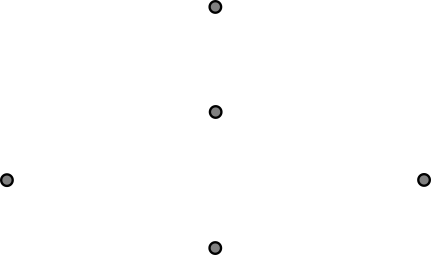
\includegraphics[width=0.85\textwidth]{figuras/vertices.png}}
            \only<2>{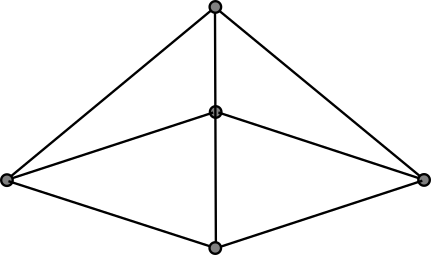
\includegraphics[width=0.85\textwidth]{figuras/arestas.png}}
            \only<3>{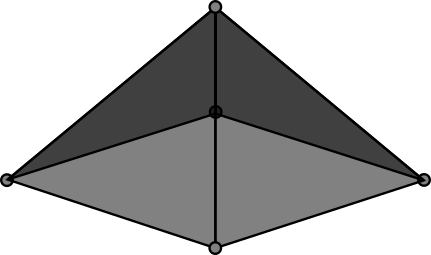
\includegraphics[width=0.85\textwidth]{figuras/faces.png}}
            \only<4>{
\includegraphics[width=0.85\textwidth]{figuras/malha.png}}
        \end{column}
    \end{columns}
\end{frame}

\section{Metodologia}

\begin{frame}{Geração Procedural}
    Para garantir uma grande quantidade de cenários de teste, foi utilizado Ruído de Perlin \cite{perlin1985image} para gerar de forma automatizada as malhas de teste \cite{patel_terrain_noise}. O algoritmo funciona empilhando múltiplas camadas ligeiramente diferentes (oitavas) de ruído para formar uma imagem contínua e suave.
    \vspace{1em}

    Em uma oitava, o espaço da imagem é dividido em uma grade e em cada interseção é atribuído um vetor de gradiente aleatório \cite{zipped_perlin_noise}. Em cada pixel da imagem, é calculado o vetor que vai dos nós da grade até esse ponto e é feita uma multiplicação escalar. Os valores calculados nos nós vizinhos são interpolados e finalmente um valor é atribuído ao pixel.
\end{frame}

\begin{frame}{Geração Procedural}
    Para que as oitavas não sejam idênticas, valores de lacunaridade (frequência) e persistência (amplitude) influenciam no cálculo dos valores finais dos pixels \cite{patel_terrain_noise}. A frequência define a quantidade de detalhes, enquanto a amplitude define a escala de intensidade desses detalhes.
    \vspace{1em}

    \begin{columns}
        \begin{column}{0.33\textwidth}
            \centering
            \scriptsize Ruído de alta frequência\\
            \vspace{0.3em}
            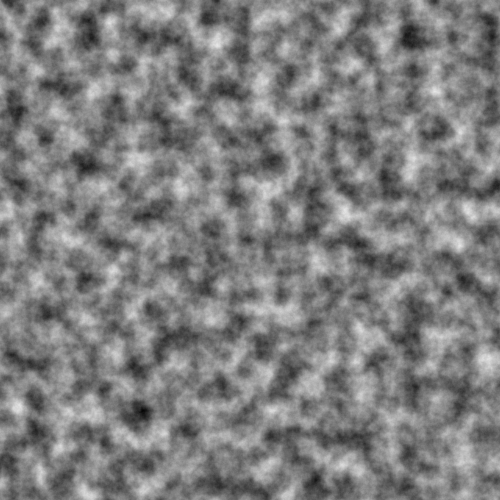
\includegraphics[width=\textwidth]{figuras/perlin_high_freq.png}
        \end{column}
        \begin{column}{0.33\textwidth}
            \centering
            \scriptsize Ruído de alta amplitude\\
            \vspace{0.3em}
            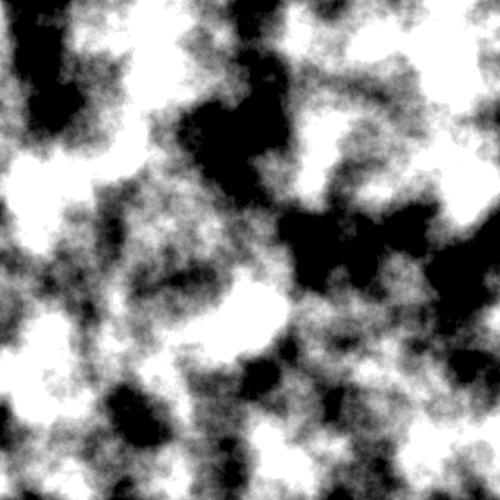
\includegraphics[width=\textwidth]{figuras/perlin_high_amp.png}
        \end{column}
        \begin{column}{0.33\textwidth}
            \centering
            \scriptsize Ruído de alta freq. e amp.\\
            \vspace{0.3em}
            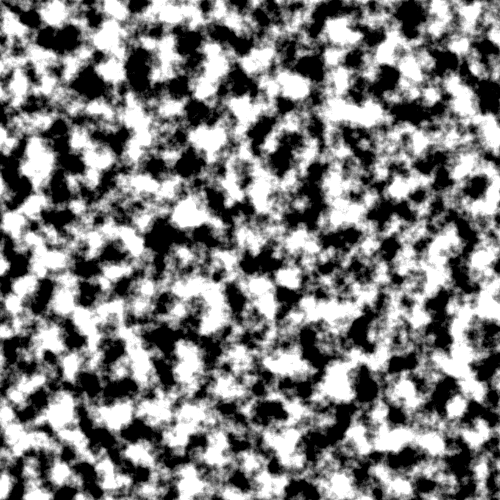
\includegraphics[width=\textwidth]{figuras/perlin_high_freq_amp.png}
        \end{column}
    \end{columns}
\end{frame}

\begin{frame}{Conversão Pixel para Vértice}
    Com uma imagem de ruído gerada, traduzem-se os valores para malha e grafo, mapeando a posição $(x, z)$ dos pixels aos vértices e convertendo o valor da cor para a altura.
    \vspace{1em}
    
    \centering
    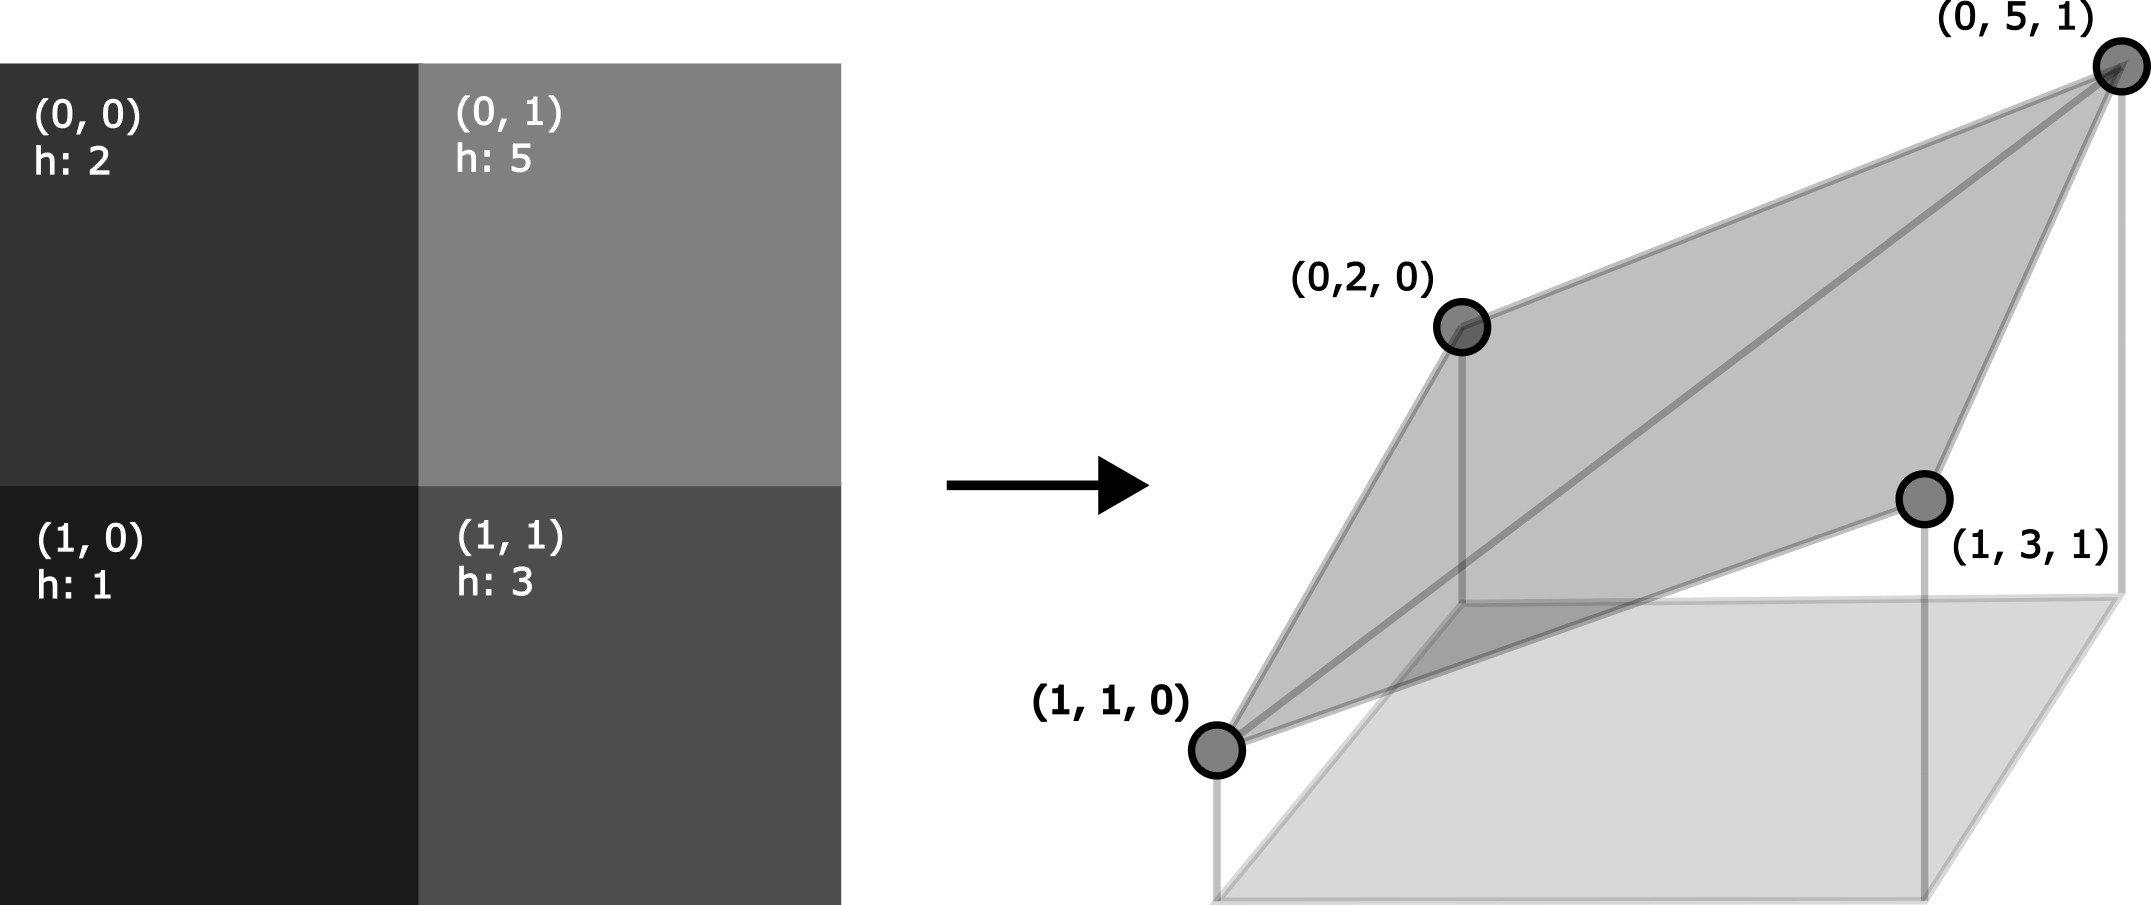
\includegraphics[width=0.85\textwidth]{figuras/pixel_to_vertex.png}
\end{frame}

\begin{frame}{Malha Resultante}
    \centering
    Exemplo de malha gerada a partir de uma imagem de ruído de Perlin.
    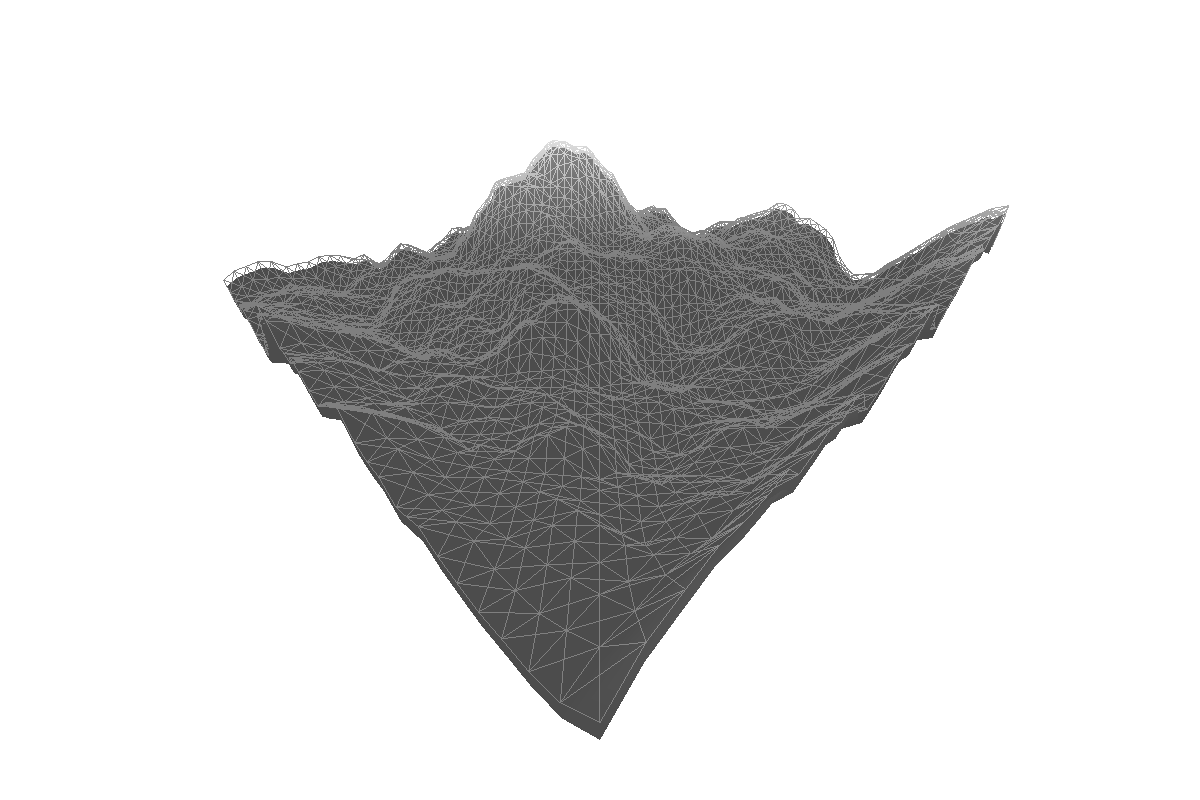
\includegraphics[width=0.7\textwidth]{figuras/mesh_from_perlin.png}
\end{frame}

\begin{frame}{Paralelização}
    \begin{columns}
        \begin{column}{0.5\textwidth}
            Todo o ambiente de teste e renderização será paralelizado pela classe \texttt{TaskMaster}. Ela encapsula conceitos de Monitor, Filas Multinível \cite{ladeira} e Task Scheduler \cite{williams2019c++}.
        \end{column}
        \begin{column}{0.5\textwidth}
            Essa arquitetura garante um ambiente concorrente limpo e seguro, executando testes enquanto o motor gráfico roda em segundo plano.
        \end{column}
    \end{columns}
    \vspace{1.5em}
    
    \centering
    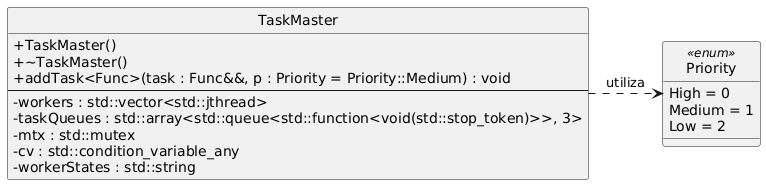
\includegraphics[width=\textwidth]{figuras/task_master.png}
\end{frame}

\begin{frame}{Desenho Experimental}
    Os algoritmos serão testados em diferentes cenários de teste, alternando entre possíveis configurações de ruídos:
    \begin{itemize}
        \item \textbf{Escala:} Tamanho da malha ($N \times N$).
        \item \textbf{Lacunaridade:} Quantidade de obstáculos.
        \item \textbf{Persistência:} Nível de dificuldade dos obstáculos.
    \end{itemize}
\end{frame}

\begin{frame}{Desenho Experimental}
    Em todos os testes serão testados:
    \begin{itemize}
        \item Tempo de CPU.
        \item Consumo de memória.
        \item Qualidade do caminho (custo).
        \item Taxa de erro de cache.
    \end{itemize}
    \vspace{1.5em}
    Será priorizado um ambiente quiescente para não haver interferências do sistema operacional \cite{lilja2000measuring, jain1991art}.
\end{frame}

\begin{frame}{Riscos Associados ao Projeto}
    \begin{table}[h]\centering
        \caption{Riscos do projeto e estratégias de mitigação}\label{tab:riscos}
        \scriptsize
        \begin{tabular}{L{3.2cm} L{7.2cm}}\toprule
        \textbf{Risco} & \textbf{Mitigação} \\\midrule
        Complexidade de adaptar algoritmos complexos como JPS 3D e Theta* & Referências de alto valor, uso de bibliotecas de teste (GTest) e otimizações de compilação \\
        \vspace{0.5em}Coleta de amostras e viés de dados & \vspace{0.5em}Controle rígido do ambiente de teste e forte embasamento teórico \\
        
        \vspace{0.5em}Expansão ambiciosa e insuficiência do tempo planejado & \vspace{0.5em}Cronograma modular, priorização de adições e ambiente de pesquisa estável \\
        \bottomrule
        \end{tabular}
    \end{table}
\end{frame}

\section{Resultados e Próximos Passos}

{\setbeamercolor{background canvas}{bg=white}
\begin{frame}[plain]
    \begin{tikzpicture}[remember picture, overlay]
        \node[fill=islamicgreen, minimum width=\paperwidth, minimum height=4cm, anchor=center] at (current page.center) {};
        \node[anchor=center, align=center] at (current page.center) {
            \color{white}\Huge\textbf{Desenvolvimento e} \\\\
            \color{white}\Huge\textbf{Resultados Parciais}
        };
    \end{tikzpicture}
\end{frame}}

\begin{frame}{Resultados Esperados}
    \begin{itemize}
        \item Distinguir melhores algoritmos para cada modelo geométrico e tipo de cenário:
        \begin{itemize}
            \item Dijkstra com pior tempo de execução (baseline).
            \item JPS com melhor tempo em áreas planas.
            \item Theta* com melhor qualidade de caminhos (any-angle).
        \end{itemize}
        \vspace{1em}
        \item Validar a influência da escala e dificuldade de terreno no tempo de execução de algoritmos de busca:
        \begin{itemize}
            \item ANOVA com $p$-valor $< 0,05$ e teste complementar de Tukey \cite{jurandir}.
        \end{itemize}
    \end{itemize}
\end{frame}

\begin{frame}{Cronograma de Atividades}
    \begin{table}[h]\centering
        \caption{Cronograma de execução das atividades}\label{tab:crono1}
        \scriptsize
        \begin{tabular}{lll}\toprule
        \textbf{Etapa} & \textbf{Período} & \textbf{Status} \\\midrule
        Revisão Bibliográfica & Jan-Fev/2026 & Concluído \\
        Motor Gráfico e Grafos & Fev-Abr/2026 & Concluído \\
        Algoritmos de Busca & Mar-Mai/2026 & Concluído \\
        Geração de Cenários & Abr-Mai/2026 & Concluído \\
        Concorrência & Mai-Jun/2026 & Concluído \\
        Planejamento da coleta de dados & Mai-Jun/2026 & Concluído \\
        Defesa do Pré-Projeto & Jun/2026 & Concluído \\
        NavMeshes, Octrees e Voxels & Jul-Set/2026 & Pendente \\
        Testes de Estresse & Ago/2026 & Pendente \\
        Algoritmos Adicionais & Ago-Set/2026 & Pendente \\
        Coleta Automatizada de Dados & Set-Out/2026 & Pendente \\
        Análise estatística & Out-Nov/2026 & Pendente \\
        Redação Final da Monografia & Out-Dez/2026 & Pendente \\
        Defesa do TCC & Dez/2026 & Pendente \\
        \bottomrule
        \end{tabular}
    \end{table}
\end{frame}

\section{Conclusão}

\begin{frame}{Considerações Finais e Conclusão}
    A elaboração do pré-projeto consolidou uma base técnica estável e demonstrou a viabilidade da pesquisa comparativa de pathfinding 3D concorrente.
    \vspace{1.5em}
    
    Principais conclusões do estágio atual:
    \begin{itemize}
        \item \textbf{Viabilidade técnica confirmada:} Motor gráfico IFCG e estruturas concorrentes (\texttt{TaskMaster}) funcionando sem instabilidades.
        \item \textbf{Rigor estatístico:} A infraestrutura e o isolamento de CPU garantem medições precisas para ANOVA.
        \item \textbf{Contribuição prática:} Desenvolvimento open-source de bibliotecas de grafos leves.
    \end{itemize}
\end{frame}

\section{Referências}
\begin{frame}[allowframebreaks]{Referências}
    \printbibliography
\end{frame}

\begin{frame}[plain]
\titlepage
\end{frame}

\end{document}